% !TEX root = ../../prj4projektdokumentation.tex
% SKAL STÅ I TOPPEN AF ALLE FILER FOR AT MASTER-filen KOMPILERES 

\section{Intern blok diagram}
Herunder på figur \ref{fig:IBDSpaendingsregulator} ses et IBD for spændingsregulator. På diagrammet ses de interne forbindelser i systemet. Under figur \ref{fig:IBDSpaendingsregulator} er en signalbeskrivelse, der uddyber diagrammet.

\begin{figure}[htbp] % (alternativt [H])
	\centering
	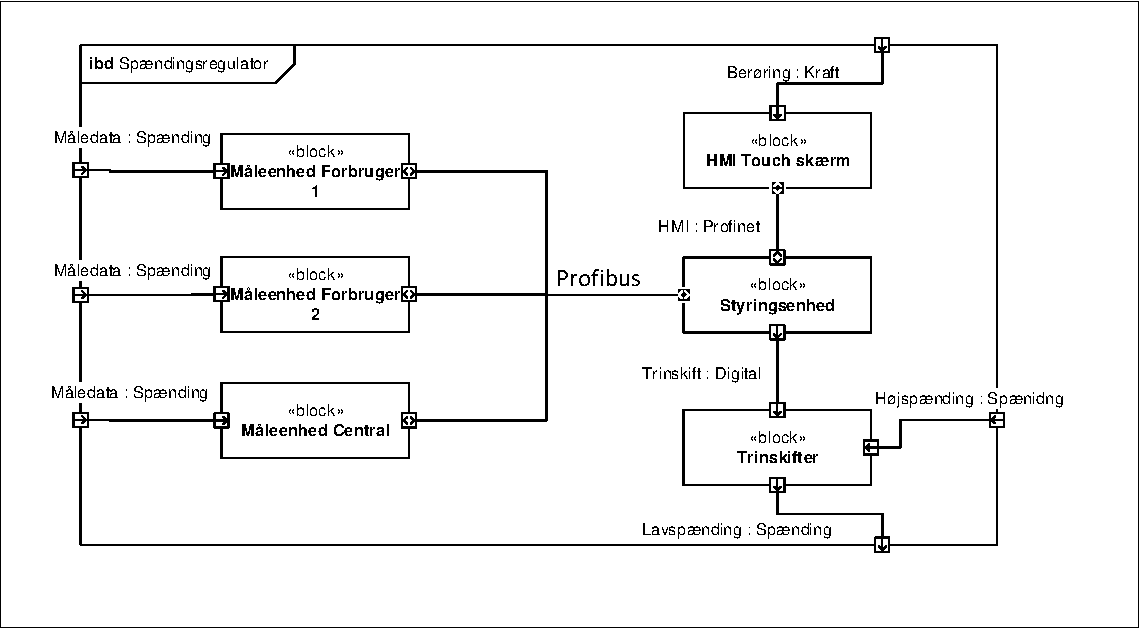
\includegraphics[width=0.8\textwidth]{Figure/IBDSpaendingsregulator}
	\caption{IBD Spændingsregulator}
	\label{fig:IBDSpaendingsregulator}
\end{figure}

\subsection{Signalbeskrivelse}

\begin{table}[htbp]
	\centering
	\begin{tabular}{|l|l|l|l|l|}
		\hline
		\textbf{Blok} & \textbf{Signal} & \textbf{Type} & \textbf{Signaltype} & \textbf{Beskrivelse} \\\hline
		\multicolumn{5}{Måleenhed Forbruger 1}} \\\cline{5-9}
 		 & Måledata	& Spænding & Måleenhed & \\\hline
		Berøring 	& Kraft & jjj & jj & ii \\\hline
		Højspænding 	& Spænding & jjj & jj & ii\\\hline
		Lavspænding 	& Spænding & jjj & jj & ii \\\hline
		Trinskift 	& Digital & jjj & jj & ii\\\hline
		HMI 	& Profinet & jjj & jj & ii \\\hline
		Profibus 	& Kommunikation & jjj & jj & ii \\\hline
		
	\end{tabular}
	\caption{Signalbeskrivelse}
	\label{tab:Signalbeskrivelse}
	
\end{table}